%&latex
%
\providecommand{\main}{../..}
\documentclass[../../main.tex]{subfiles}

\begin{document}

\subsection{Extinction time distribution}\label{sec:extintion-times}
\lesson{32}{21/05/20}

Let's return to the simplest case, with no density dependence ($\tilde{d} = \tilde{b} = 0$), closed boundaries ($b_0 = 0$) and per-capita birth-death rates proportional to population ($b_n = n b$ and $d_n = n d$ for $n \geq 1$).

\medskip

In this scenario, when a certain species reaches the $n=0$ state, it becomes \textbf{extinct}. Let $\mathcal{P}(t|n_0)\dd{t}$ be the probability that a species starting with $n_0$ individuals gets extinct at a time in $(t, t+\dd{t})$.  To compute $\mathcal{P}(t|n_0)$ we have to solve the Master Equation (\ref{eqn:birth-death-ME}):
\begin{align}\label{eqn:birth-death-ME2}
    \dot{\mathbb{P}}_{n} = {(n-1)b\,\mathbb{P}_{n-1}(t)} + {(n+1)d\,\mathbb{P}_{n+1}(t) }- n(b+d) \mathbb{P}_n(t) \qquad n\geq 0
\end{align}
with $\mathbb{P}_{-1} \equiv 0$.

\medskip

To do this, we use the \textit{probability} generating function $G(z,t)$ of $\mathbb{P}_n(t)$:
\begin{align*}
    G(z,t) = \sum_{n=0}^{+\infty} \mathbb{P}_n(t) z^n 
\end{align*} 
Recall that $G(1,t) \equiv 1$ $\forall t$ due to normalization.

\medskip

So, if we multiply both sides of (\ref{eqn:birth-death-ME2}) by $z^n$ and sum over $z$ we get:
\begin{align*}
    \underbrace{\sum_{n=0}^{+\infty} \dot{\mathbb{P}}_n(t) z^n}_{\dot{G}(z,t)}  &= b\sum_{n=0}^{+\infty} (n-1) \mathbb{P}_{n-1}(t) z^n + d\sum_{n=0}^{+\infty} (n+1) \mathbb{P}_{n+1}(t) z^n - (b+d)\sum_{n=0}^{+\infty} n \mathbb{P}_n(t) z^n
\end{align*}
Note that, by shifting the indeces of summation:
\begin{align*}
    \sum_{n=0}^{+\infty} n \mathbb{P}_n(t) z^n &= z\partial_z G(z,t)\\
    \sum_{n=0}^{+\infty} z^n(n-1) \mathbb{P}_{n-1}(t) &= \sum_{n=\textcolor{Red}{1}}^{+\infty} z^{n\textcolor{Red}{+1}} n \mathbb{P}_n(t) = z \sum_{n=\textcolor{Red}{0}}^{+\infty} n z^n \mathbb{P}_n = z^2 \partial_z G(z,t)\\
    \sum_{n=0}^{+\infty} z^n(n+1) \mathbb{P}_{n+1}(t) &= \sum_{n=0}^{+\infty} z^{n-1} n \mathbb{P}_n(t) = \partial_z G(z,t)
\end{align*}
Substituting back:
\begin{align*}
    \partial_t G(z,t) &= b z^2 \partial_z G(z,t) + d \partial_z G(z,t) - (b + d) z \partial_z G(z,t) =\\
    &= [b z^2 - (b+d)z + d]\partial_z G(z,t) = (bz - d)(z-1) \partial_z G(z,t)
\end{align*}
So at the end we have to solve:
\begin{align}\label{eqn:extinction-diffeq}
    \partial_t G(z,t) = (bz - d) (z-1) \partial_z G(z,t)
\end{align}
Note that for $z=1$, $\partial_t G(1,t) \equiv 0$, which is consistent with $G(1,t) = 1$ $\forall t$.
%Initial condition will come back later on


This equation may be solved with the method of characteristics. We start by parametrizing $z\colon [0,t] \ni \tau \mapsto z(\tau)$ as follows:
\begin{align}\label{eqn:z-tau}
    \dot{z}(\tau) = -(b z(\tau) - d) (z(\tau) - 1)
\end{align}
which is just $-\partial_t G(z(\tau),t)$. 

Now, if we compute the total derivative of $G(z,t)$ \textit{along} the curve $z(\tau)$ we get:
\begin{align*}
    \dv{\tau} G(z(\tau), \tau) &= [\partial_\tau G(z,\tau) + \dot{z}(\tau) \partial_z G(z, \tau)]_{z=z(\tau)} =\\
    &= \left[\pdv{\tau} G(z,\tau) - (bz - d)(z-1) \pdv{z} G(z,\tau)\right]_{z = z(\tau)} \underset{(\ref{eqn:extinction-diffeq})}{=} 0
\end{align*} 
Thus:
\begin{align}\label{eqn:G-along-curve}
    G(z(\tau), \tau) = \text{Constant} = G(z(0), 0) \qquad \forall \tau
\end{align}
Let's fix the initial population to $n_0$, meaning that $\mathbb{P}_n(t=0) = \delta_{n,n_0}$. Then:
\begin{align*}
    G(z,t=0) = \sum_{n=0}^{+\infty} \delta_{n, n_0} z^n = z^{n_0}
\end{align*}
and in particular $G(z(0),0) = z(0)^{n_0}$. 

\medskip

As we want to compute $G(z,t)$, we fix the \textit{endpoint} of $z(\tau)$ to be $z(t) \overset{!}{=} z$. Then (\ref{eqn:G-along-curve}) evaluated at $t$ reads:
\begin{align}\label{eqn:G-z-t}
    G(z(\tau), \tau) \Big|_{\tau = t} = G(z(t), t) = G(z, t) = G(z(0), 0) = z(0)^{n_0}
\end{align}

The starting point $z_0(0)$ will depend in general on both $z$ and $t$, and can be determined by solving the differential equation (\ref{eqn:z-tau}), which is an ordinary differential equation that may be solved by separation of variables:
\begin{align*}
    \dot{z}(\tau) &= - (z(\tau) - 1)(b z(\tau) - d)\\
    \dd{z} \left(\frac{1}{1-z} + \frac{b}{bz -d}  \right) &= \dd{\tau} (b-d)\\
    \int_{z(0)}^z \left(\frac{1}{1-z} + \frac{b}{bz -d}  \right)\dd{z} &= - t(d-b)
\end{align*}
Notice that $bz-d < 0$ since we are interested to $z \in [0,1]$ and $b < d$. Computing the integral leads to:
\begin{align*}
    \ln \left| \frac{d-bz}{1-z} \frac{1-z(0)}{d-bz(0)}  \right| = -(d-b) t
\end{align*}
which can be solved for $z(0)$, resulting in:
\begin{align*}
    z(0) = \frac{1 - dA}{1-bA} \qquad A \equiv \frac{1-z}{d-bz} e^{-(d-b)t}  
\end{align*}
Substituting back in (\ref{eqn:G-z-t}) we obtain the solution:
\begin{align}\label{eqn:extinction-generating}
    G(z,t) = \left(\frac{1-dA}{1-bA} \right)^{n_0}
\end{align}
Notice that when $z=1$, $A=0$ and so $G(1,t) = 1$ as expected.

\medskip

Recall that:
\begin{align*}
    G(z,t) = \mathbb{P}_0(t) + z \mathbb{P}_1(t) + z^2 \mathbb{P}_2(t) + \dots
\end{align*}
In particular, $\mathbb{P}_0(t)$ is the probability that a certain species has a population $0$ at time $t$, meaning that it became extinct at a time $t_0 \leq t$. Note that:
\begin{align*}
    G(0,t) = \mathbb{P}_0(t)
\end{align*}

\medskip

Conversely, the probability $\mathcal{P}_>(t|n_0)$ that a species is still alive at time $t$, i.e. that it will become extinct at a time $t_0 > t$ is given by:
\begin{align*}
    \mathcal{P}_>(t|n_0) = 1 - \mathbb{P}_0(t)
\end{align*}

Using (\ref{eqn:extinction-generating}), we have:
\begin{align*}
    A\Big|_{z=0} = \frac{1}{d} e^{-\delta t}; \quad \delta = d-b > 0  \Rightarrow G(0,t) = \left[\frac{1 - e^{-\delta t}}{1 - (b/d) e^{-\delta t}} \right]^{n_0} = \left[1 + \frac{\delta}{d} \frac{e^{-\delta t}}{1 - e^{-\delta t}}  \right]^{-n_0}
\end{align*}
Thus:
\begin{align}\label{eqn:lifetime-pdf}
    \mathcal{P}_>(t|n_0) &= 1- \mathbb{P}_0(t) = 1 - G(0,t) = 1 - \left[1- \frac{\delta}{d} \frac{e^{-\delta t}}{1 - e^{-\delta t}}  \right]^{-n_0}
\end{align}

We can finally compute the extinction time distribution. Let $\mathcal{P}(t|n_0) \dd{t}$ be the probability that a species with $n_0$ individuals becomes extinct at time in $(t, t+ \dd{t})$. This is merely the probability of surviving until $t$, but not after $t+ \dd{t}$:
\begin{align}\label{eqn:lifetime-derivative}
    \mathcal{P}(t|n_0)\dd{t} = \mathcal{P}_>(t|n_0) - \mathcal{P}_>(t+\dd{t}|n_0) = - \dd{t} \pdv{t} \mathcal{P}_>(t|n_0)
\end{align}
Dividing by $\dd{t}$ we get:
\begin{align}\label{eqn:extinction-diff-eq}
    \mathcal{P}(t|n_0) = -\pdv{t} \mathcal{P}_>(t|n_0)
\end{align}


Before computing (\ref{eqn:extinction-diff-eq}), let's try to simplify a bit more (\ref{eqn:lifetime-pdf}). In particular, we are interested in its \textit{scaling behaviour} near the \q{critical point} $\delta \approx 0$.

\medskip

From empirical observations, $\delta \ll \SI{1}{y^{-1}}$ for forests. Its reciprocal defines an \textit{emergent} timescale $\tau_c$:
\begin{align}\label{eqn:tau-c}
    \tau_c \equiv \frac{1}{\delta}  \gg \SI{1}{y}
\end{align} 
In particular, $\tau_c \sim \SI{e3}{y}$. Physically, $\tau_c$ represents the \textit{relaxation time} needed by a forest to recover from a small perturbation. 

\medskip

If we take $\delta \cdot t$ fixed and let $\delta \to 0$, then (\ref{eqn:lifetime-pdf}) becomes:
\begin{align*}
    \mathcal{P}_>(t|n_0) &= 1-\left[1+\frac{\delta}{d} \frac{e^{-\delta t}}{1 - e^{-\delta t}}  \right]^{-n_0} = \frac{n_0 \delta}{d} \frac{e^{-\delta t}}{1 - e^{-\delta t}} =\\
    &= \frac{n_0 \delta}{d} (e^{\delta t} - 1)^{-1} \equiv \frac{n_0}{d \cdot t} F(\delta \cdot t)  \\
    F(x) &= \frac{x}{e^x -1} \to \begin{cases}
        1 & x \to 0\\
        0 & x \to \infty
    \end{cases}
\end{align*}
So for $\delta \to 0$:
\begin{align*}
    \mathcal{P}_>(t|n_0) \sim \begin{cases}
        t^{-1} & t \cdot \delta \ll 1 \mathrm{\ i.e.\ } t \ll \tau_c\\
        e^{-t/\tau_c} & t \gg \tau_c
    \end{cases}
\end{align*}
This implies that the lifetime distribution (\ref{eqn:extinction-diff-eq}) has the following scaling:
\begin{align}\label{eqn:lifetime-dist}
    \mathcal{P}(t|n_0) &= \frac{1}{t^2} f(t/\tau_c) \frac{n_0}{d}\\ \nonumber
    f(x) &= F(x) - xF'(x) = \frac{x^2 e^x}{(e^x - 1)^2} \to \begin{cases}
        1 & x \to 0\\
        0 & x \to \infty
    \end{cases} \\ \nonumber
    \Rightarrow \mathcal{P}(t|n_0) &\sim \begin{cases}
        t^{-2} & t \ll \tau_c\\
        e^{-t/\tau_c} & t \gg \tau_c
    \end{cases}
\end{align}

A plot of $\mathcal{P}(t|n_0)$ is shown in fig. \ref{fig:lifetime-dist}.

\begin{figure}[H]
    \centering
    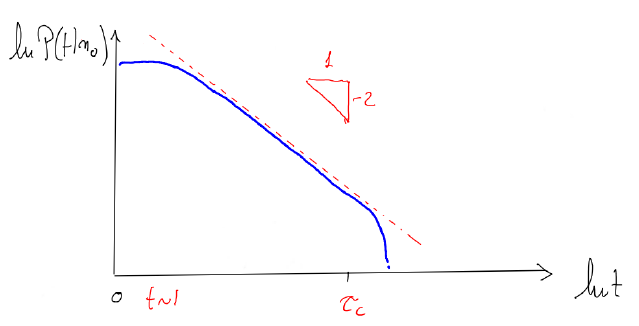
\includegraphics[width=0.8\textwidth]{\main/Images/lifetime-dist.png}
    \caption{Log-log plot of the extinction time (or lifetime) distribution $\mathcal{P}(t|n_0)$.}
    \label{fig:lifetime-dist}
\end{figure}

This can be compared with real data - with some difficulties given that \textit{fossil records} are not very accurate, and good records have usually a duration of less than $\SI{50}{y}$. For example, if we consider birds species, we can see different scenarios (top of fig. \ref{fig:birds}):
\begin{enumerate}
    \item A species emerges and disappears entirely within the span of observations (blue plot).
    \item A species is initially present from a un unknown time, then disappears from that region, only to return and disappear again after some time (orange plot).
    \item A species is already present at the start of observations, and never disappears.
\end{enumerate}
In the first two cases we can estimate the lifetimes $\tau'$ of these two species, but in the third we can only give a lower bound $\tau''$ for it. With some manipulations, we can use (\ref{eqn:lifetime-dist}) to produce theoretical predictions, which fit well the available data (fig. \ref{fig:birds}).

\begin{figure}[H]
    \centering
    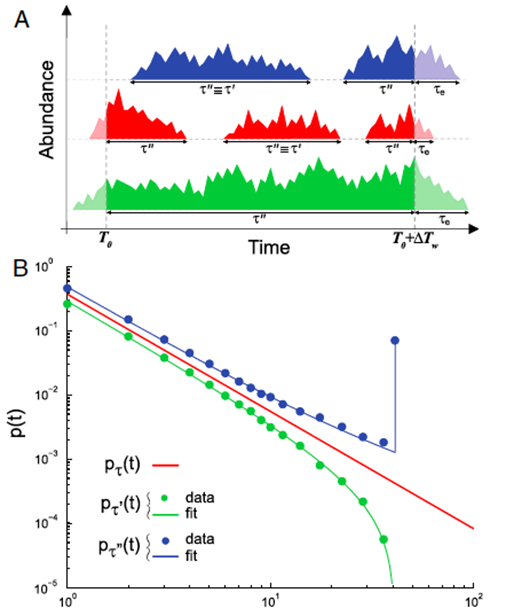
\includegraphics[width=0.7\textwidth]{\main/Images/birds.png}
    \caption{The window available for observations has a limited duration, meaning that we cannot measure directly lifetimes of species $\tau$. What we can know are only the lifetimes that happen within the window ($\tau'$), or lower bounds for lifetimes larger than the window ($\tau''$). So, we cannot use directly (\ref{eqn:lifetime-dist}) for a fit, but need to account for these limitations - leading to the blue and green lines. Still, the model follows well the real data (blue and green points).}
    \label{fig:birds}
\end{figure}


%Presentation continues
\subsection{Continuum limit}\label{sec:birth-death-continuum}
Recall the Master Equation (\ref{eqn:birth-death-ME2}) and let $x = n$ and $\mathbb{P}_n = p_x$:
\begin{align*}
    \pdv{p_x(t)}{t}=b(x-1) p_{x-1}(t)+d(x+1) p_{x+1}(t)-[b(x)+d(x)] p_{x}(t)
\end{align*}
If we treat $x$ as a continuous variable (in the limit of a large population) we can expand $p_{x\pm1}$, leading to:
\begin{align}\label{eqn:me-fokker-planck}
    \pdv{p(x,t)}{t} = \pdv{x} [d(x) - b(x)] p(x,t) + \frac{1}{2} \pdv[2]{x} [d(x) + b(x)] p(x,t) 
\end{align}
which looks like a Fokker-Planck equation with diffusion coefficient $D = [d(x) + b(x)]/2$.

Then, if we take:
\begin{align*}
    b(x) = b_1 x + b_0\qquad d(x) = d_1 x - b_0
\end{align*}
Equation (\ref{eqn:me-fokker-planck}) may be rewritten as:
\begin{align}\label{eqn:modelpde}
    \dot{p} = \partial_x[(x/\tau - b)p] + D\partial_x^2 (xp) \qquad \begin{cases}
        D = \frac{d_1 + b_1}{2}\\
        \tau = \frac{1}{d_1 - b_1} > 0\\
        b = 2b_0 > 0  
    \end{cases}
\end{align}
which is equivalent to the following Langevin equation:
\begin{align*}
    \dot{x}(t) = b - x(t)/\tau + \sqrt{D x(t)} \xi(t)
\end{align*}
The term $b$ quantifies the \textit{immigration} rate, $x(t)/\tau$ is the rate of population decay (since $d_1$ is slighty over $b_1$) and $\xi(t)$ represents the stochastic fluctuations with amplitude $\sqrt{D x(\tau)}$.

\medskip

Equation (\ref{eqn:modelpde}) may be solved by using standard techniques for PDE\textit{s}, resulting in:
\begin{align*}
    p(x, t | x_{0}, 0) = &\left(\frac{1}{D \tau}\right)^{\frac{b}{D}} x^{\frac{b}{D}-1} e^{-\frac{x}{D \tau}} \frac{\left[\left(\frac{1}{D \tau}\right)^{2} x_{0} x e^{-t / \tau}\right]^{\frac{1}{2}-\frac{b}{2 D}}}{1-e^{-t / \tau}} \times \\
    & \times \exp \left[-\frac{\frac{1}{D \tau}\left(x+x_{0}\right) e^{-t / \tau}}{1-e^{-t / \tau}}\right] I_{\frac{b}{D}-1}\left[\frac{2 \frac{1}{D \tau} \sqrt{x_{0} x e^{-t / \tau}}}{1-e^{-t / \tau}}\right]
\end{align*}
Here we used \textit{reflecting} boundary conditions at $x=0$.

\medskip

The stationary state is given by a $\Gamma$ distribution:
\begin{align*}
    p(x,t|x_0,0) \xrightarrow[t \to \infty]{} p_{0}(x)=(D \tau)^{-b / D} \Gamma(b / D)^{-1} x^{\frac{b}{D}-1} e^{-\frac{x}{D \tau}}
\end{align*}
and agrees well with data (fig. \ref{fig:gamma-stat}).

\begin{figure}[H]
    \centering
    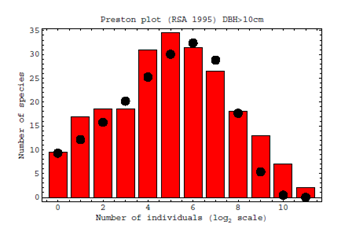
\includegraphics[width=0.7\textwidth]{\main/Images/gamma-stat.png}
    \caption{Fit of RSA data with a $\Gamma$ distribution.}
    \label{fig:gamma-stat}
\end{figure}

We can also compute the \textit{species turnover} distribution, i.e. the probability of a certain species having a population $x$ at time $t$ such that $x/x_0 = \lambda$ for a given $\lambda$:

\begin{align} \nonumber
    \mathcal{P}_{\mathrm{STD}}(\lambda, t)=&\left\langle\delta\left(\lambda-x / x_{0}\right)\right\rangle \\ \nonumber
    =& \int_{0}^{\infty} \dd{x_0} \int_{0}^{\infty} \dd{x} p\left(x, t | x_{0}, 0\right) p_{0}\left(x_{0}\right) \delta\left(\lambda-x / x_{0}\right) \\
    \nonumber
    =& \frac{2^{\frac{b}{D}-1}}{\sqrt{\pi}} \frac{\Gamma\left(\frac{b}{D} + \frac{1}{2}  \right)}{\Gamma\left(\frac{b}{D} \right)} \frac{(\lambda + 1)}{\lambda} \frac{(e^{t/\tau}) e^{\frac{b}{2D}}}{1 - e^{-t/\tau}} \left(\frac{\sinh \left(\frac{t}{2 \tau} \right)}{\lambda} \right)^{\frac{b}{D}+1 }   \\ \label{eqn:species-turnover}
    & \times\left(\frac{4 \lambda^{2}}{(\lambda+1)^{2} e^{t / \tau}-4 \lambda}\right)^{\left(\frac{b}{D} + \frac{1}{2} \right)}
\end{align}

By fitting the stationary state distribution we can determine $2$ parameters out of $3$: $b$ and $D$, but not $\tau$. Then $\tau$ can then be determined by fitting the species turnover distribution (fig. \ref{fig:speciesturnover})

\begin{figure}[H]
    \centering
    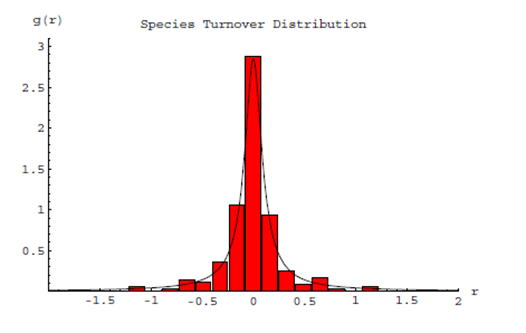
\includegraphics[width=0.7\textwidth]{\main/Images/speciesturnover.png}
    \caption{Fit of (\ref{eqn:species-turnover}) to determine $\tau \sim \SI{3400}{y}$ for a tropical forest.}
    \label{fig:speciesturnover}
\end{figure}

\section{Spatial models}\label{sec:spatial-models}
Until now we completely neglected \textit{spatial effects} in the data, i.e. the physical distribution of species in the environment. 

One of the main models that includes these kinds of features is the \textbf{voter model}, originally created to understand elections and \textit{influences} between different voters.

The main idea is the following:
\begin{itemize}
    \item Consider, for simplicity, a square lattice. Each individual (e.g. tree) occupies one node in the lattice, meaning that the density of individuals is fixed (as it is empirically known).
    \item At each timestep, a node $x$ is chosen at random and \textit{removed}. Then:
    \begin{itemize}
        \item With probability $1-\nu$ a randomly chosen neighbour of $x$ gives birth to a new individual replacing the removed one.
        
        This mimics the fact that, when a tree dies, its place will be colonized by one of the neighbouring trees.  
        \item With probability $\nu$, the place of $x$ will be taken instead by a individual of a \textbf{new species}. This represents the effect of \textit{random mutations}.  
    \end{itemize}
\end{itemize}

A simulation of this kind of process will look like this:
\begin{figure}[H]
    \centering
    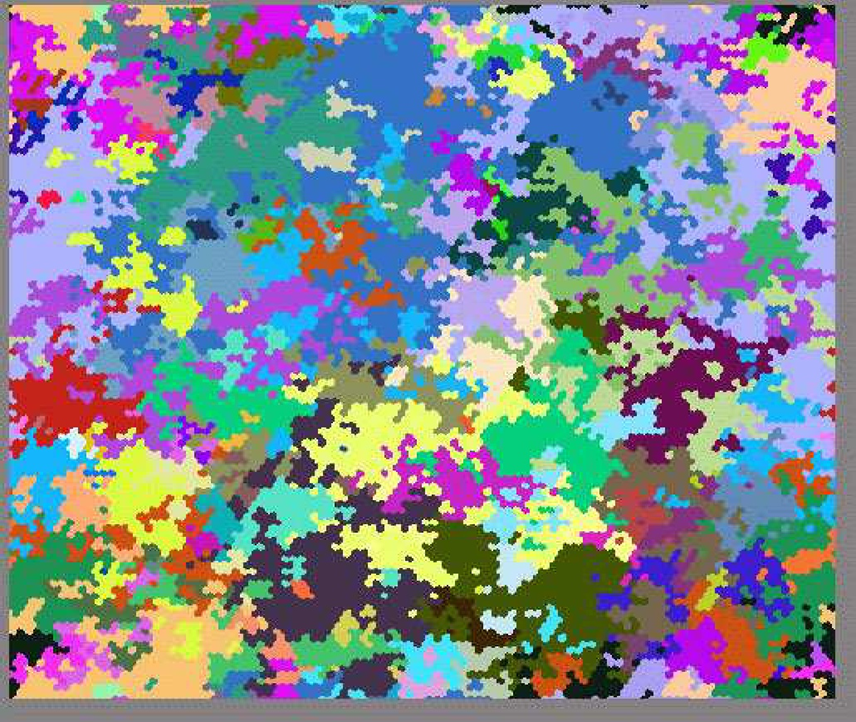
\includegraphics[width=0.7\textwidth]{\main/Images/voter-sim.png}
    \caption{Voter model simulation on a exagonal grid. Each color represents a different species.}
    \label{fig:voter-sim}
\end{figure}

We can then measure the $\beta$-diversity, i.e. the probability $F_r$ that two individuals at a distance $(r,r+\dd{r})$ belong to the same species. Empirical data shows that $F_r$ follows two different scaling regimes depending on $r$ (fig. \ref{fig:beta-div}). Our goal is then to replicate this behaviour with a voter model.

\begin{figure}[H]
    \centering
    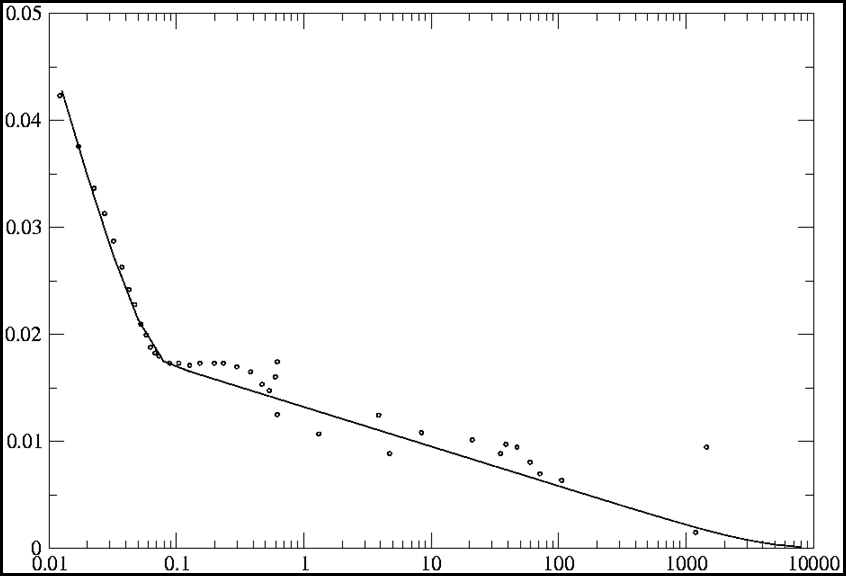
\includegraphics[width=0.6\textwidth]{\main/Images/beta-div.png}
    \caption{Probability that two individuals at distance $r$ belong to the same species. The black dots are real data from the Yasuni forest. Our target is to find a model able to predict the fitting black line.}
    \label{fig:beta-div}
\end{figure}

\medskip
%TODO As we will see?
Explicitly, two trees that are separated by a vector $\bm{x}$ are of the same species at step $n$ with probability $F_{\bm{x}}^{n}$, which evolves in a \textit{basic} voter model according to:
\begin{align}\label{eqn:beta-evo}
    F_{\bm{x}}^{n+1} = F_{\bm{x}}^n \left(1 - \frac{2}{N} \right) + \frac{1-\nu}{d N} \sum_{\mu=1}^d (F_{\bm{x} + \bm{\hat{\mu}}}^n + F_{\bm{x} - \bm{\hat{\mu}}}^n) 
\end{align}
At stationarity:
\begin{align*}
    F_{\bm{x}} &= \left(\int_{-\pi < q_i < +\pi} \frac{\dd[d]{\bm{q}}}{(2\pi)^d} \frac{1}{l(\bm{q})}  \right)^{-1} \int_{-\pi < p_i < +\pi} \frac{\dd[d]{\bm{p}}}{(2\pi)^d} e^{i \bm{p} \cdot \bm{x}} \frac{1}{l(\bm{p})}\\
    l(\bm{p}) &= -\frac{2}{N} + 2 \frac{1-\nu}{d N} \sum_{\mu=1}^d \cos(p_\mu)  
\end{align*}

In $d = 1$, the stationary solution has a purely exponential decay (fig. \ref{fig:stat-beta-decay}):
\begin{align*}
    F_r &= e^{-r/\xi}\\
    \xi &= \left(\ln \frac{1-\nu}{1 - \sqrt{\nu(2-\nu)}} \right)^{-1} \underset{\mathclap{\nu \to 0}}{\approx} \> \nu^{-1/2}
\end{align*}
This is clearly not the behaviour we need to fit fig. \ref{fig:beta-div}. 

\begin{figure}[H]
    \centering
    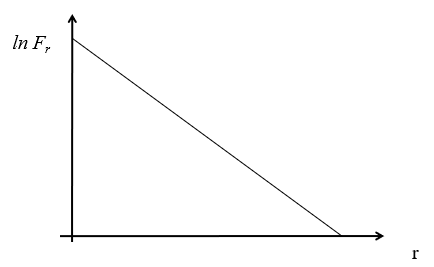
\includegraphics[width=0.7\textwidth]{\main/Images/stat-beta-decay.png}
    \caption{The decay of $F_r$ at stationarity in $d=1$ is purely exponential.}
    \label{fig:stat-beta-decay}
\end{figure}

Let's try again in a higher dimension. In $d=2$ a solution can be found by taking the continuum limit of (\ref{eqn:beta-evo}):
\begin{align*}
    \dot{F}(\bm{x},t) = \nabla^2 F(\bm{x},t) - \gamma^2 F(\bm{x},t) + s \delta^d(\bm{x})
\end{align*}
where $\gamma^2 = 2d \nu/a^2$, $a$ is the lattice spacing ($\sim \mathrm{density}^{-1/2}$), and $s$ is a free parameter. At stationarity this leads to:
\begin{align}\label{eqn:f0}
    F_0(r) = \frac{s \gamma^2}{2 \pi} K_0(\gamma r) \approx \begin{cases}
        - \frac{s \gamma^2}{2 \pi} \ln (\gamma r) & \gamma r \ll 1\\
        \frac{s \gamma^2}{2} \sqrt{\frac{1}{2 \pi \gamma r} }   e^{-\gamma r} & \gamma r \gg 1
    \end{cases} 
\end{align}
where $K_p$ is the \textit{modified} Bessel $K$ function of order $p$. 

A plot of $F_0(r)$ in $d=2$ is shown in fig. \ref{fig:beta-2} and compared from results from simulations. Again, the results are different from fig. \ref{fig:beta-div}, and in particular there is only \textit{one regime}. 

\begin{figure}[H]
    \centering
    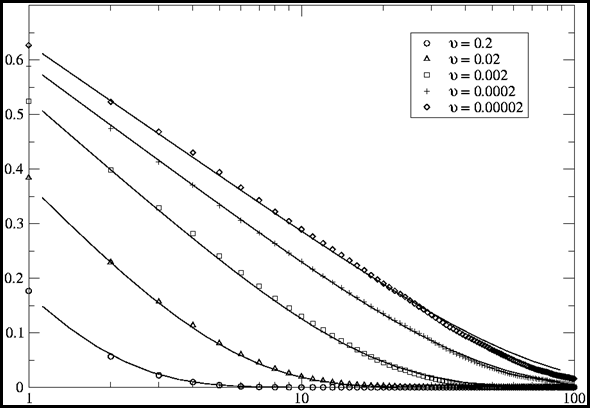
\includegraphics[width=0.7\textwidth]{\main/Images/beta-2.png}
    \caption{Plot of the $\beta$-diversity $F_0(r)$ in $d=2$ (\ref{eqn:f0}) for various values of the mutation rate $\nu$ (black continuous lines). The points are results from numerical simulations.}
    \label{fig:beta-2}
\end{figure}

These results indicate that a basic voter model is not able to explain by itself the \textit{two regimes} seen in fig. \ref{fig:beta-div}. Thus, we need to introduce \q{by hand} a strong \textit{negative} density-dependence. This is the so-called Jenzen-Connell effect, stating that:
\begin{itemize}
    \item A young tree near an adult of the same species is more likely to die than a isolated one
    \item A seedling near an adult tree of the same species is more likely not to germinate than an isolated one
\end{itemize}
Possible explanations involve the fact that trees of the same species are vulnerable from the same pests - meaning that an \q{infected} adult tree can negatively affect neighbouring young trees of the same species. Another possibility is that trees emit waste products that are \textit{toxic} for other conspecific trees. 

\medskip

So, let $p_d(x)$ be the probability that a newborn tree dies out when there is an adult tree at distance $x$. This leads to the following modification for the voter model:
\begin{align*}
    \dot{F}(\bm{x},t) &= 2\left(D \nabla^2 F(\bm{x},t) - \frac{\alpha}{1-p_d(\bm{x})} F(\bm{x},t) \right) + 2 \frac{b}{1-p_d(\bm{x})} \delta^d(\bm{x})\\
    \alpha_e &\equiv \frac{\alpha}{1-p_d(\bm{x})}  = \begin{cases}
        \alpha_0 & \norm{\bm{x}} < R\\
        \alpha_1 & \norm{\bm{x}} > R
    \end{cases} \qquad \alpha_0 > \alpha_1
\end{align*}
At stationarity:
\begin{align*}
    F_0(r) = \begin{cases}
        \frac{s \gamma_0^2}{2 \pi} K_0(\gamma_0 r) + c_1 I_0(\gamma_0 r) & r < R\\
        c_2 K_0(\gamma_1 r) & r > R 
    \end{cases}
\end{align*}
And this finally allows to replicate the behaviour of fig. \ref{fig:beta-div}.
 
%TODO Add final summary (final slide)











\end{document}